\documentclass{article}

\usepackage[english]{babel}
\usepackage[utf8]{inputenc}
\usepackage{amsmath,amssymb}
\usepackage{parskip}
\usepackage{graphicx}

% Margins
\usepackage[top=2.5cm, left=2.5cm, right=2.5cm, bottom=4.0cm]{geometry}

%%%%%%%%%%%%%%%%%
%     Title     %
%%%%%%%%%%%%%%%%%
\title{Laboratorio 4 - Inteligencia Artificial}
\author{Brenner Hernandez \\ 1023718}
\date{\today}

\begin{document}
\maketitle

%%%%%%%%%%%%%%%%%
%   Serial      %
%%%%%%%%%%%%%%%%%
\section{Serial}

% Example of how to add figure (can be used for jpeg, png, pdf, eps etc)
\begin{figure}[h!]
    \centering
    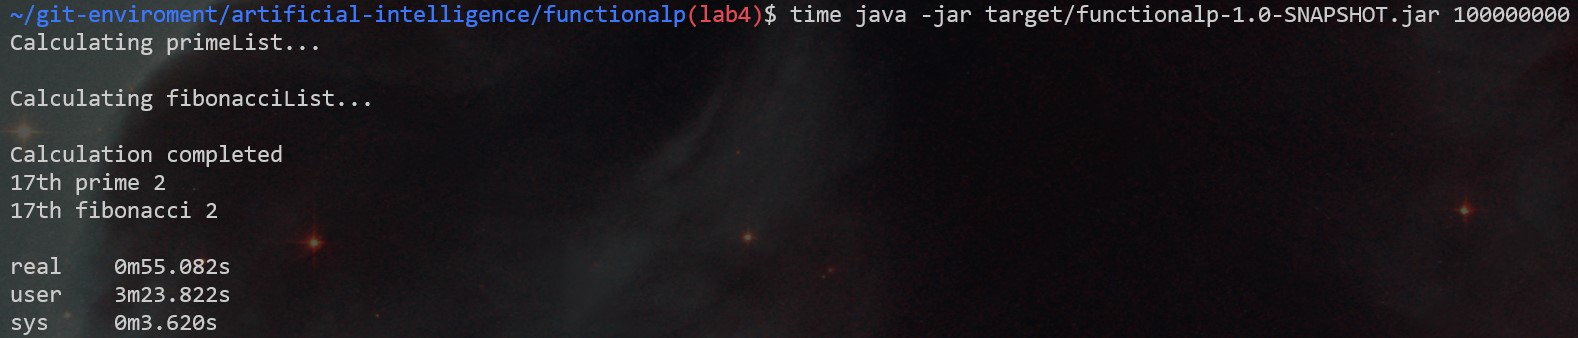
\includegraphics[width=1.0\textwidth]{serial.jpg}
    \label{fig:serial}
\end{figure}


%%%%%%%%%%%%%%%%%
%   Paralela    %
%%%%%%%%%%%%%%%%%
\section{Paralela}

% Example of how to add figure (can be used for jpeg, png, pdf, eps etc)
\begin{figure}[h!]
    \centering
    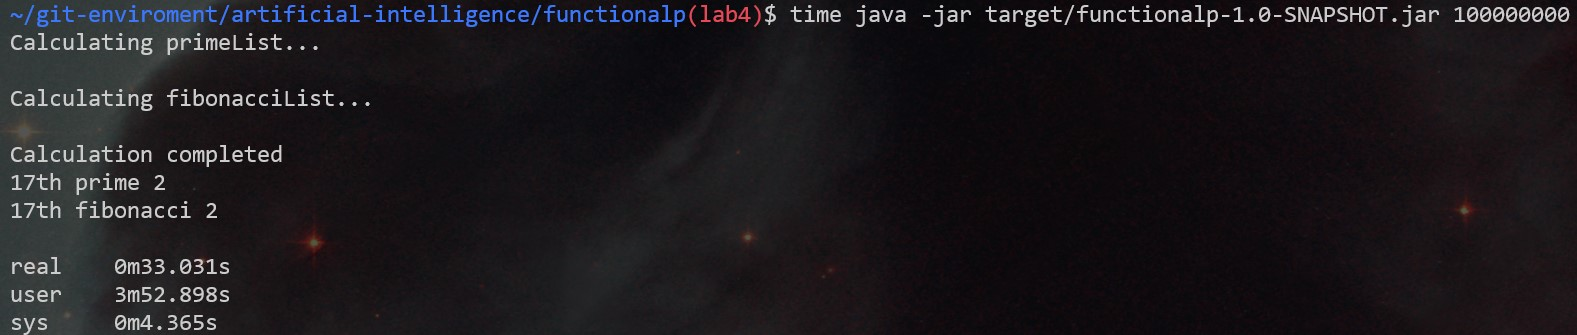
\includegraphics[width=1.0\textwidth]{parallel.jpg}
    \label{fig:parallel}
\end{figure}
%%%%%%%%%%%%%%%%%
%   ¿Mejora el tiempo de ejecución? ¿Por qué?    %
%%%%%%%%%%%%%%%%%
\section{¿Mejora el tiempo de ejecución? ¿Por qué?}
\paragraph{}{\large Sí mejora. Esto se deba a que en el stream paralelo, tanto en la generación de los números aleatorios, como el mapeo de cada uno de ellos a la nueva lista con el enésimo número de la sequencia de fibonacci; los threads disponibles para este proceso, trabajan al mismo tiempo, indicado por el \texttt{parallelStream()}, y por lo tanto se reduce el tiempo de ejecución.}

\end{document}
